\addchapheadtotoc
\chapter{Evaluation}
\label{evaluation}

This chapter gives an evaluation of feasibility for each of the implemented microservices and points out pitfalls and drawbacks as well as advantages. A final outlook lists elements of concern that need to be covered in future efforts to leverage the full potential of the automation system.

\section{Azure Microservice}
The policy evaluation and compliance service of Azure already provide all the functionality required to test the system resources. Running additional tests on the \enquote{correctness} of their evaluations would be a waste of time. A second advantage of delegating the evaluation to a thoroughly tested cloud service is the high confidence we can assign for \enquote{Passed} or \enquote{Failed} tests. 
Since the implementation of this PoC has no underlying SLAs (Service Level Agreements), even the run-time of the Azure microservice can be neglected.

However, uncovering potential lengthy running evaluations and providing an indication of possible wait times when running the automated testing pipeline can be of great value for the evaluation of the feasibility of using the Azure microservice in production. Therefore, some runtime tests have been made by executing the same evaluation on the same system ten times. The tests were conducted on the currently used Azure Subscription of the security team at ETAS SEC/ECT-Fe with 176 to be evaluated policies active in the compliance scope. According to \citep{stackoverflowTrigger}, only executing a single compliance check of a given policy is possible. This, however, has to be investigated further outside the scope of this thesis. 

\begin{table}[htb]
\begin{tabular}{|l|l|l|l|l|l|l|l|}
\hline
\textbf{Run} & \textbf{Init} & \textbf{Def} & \textbf{Assign} & \textbf{Trigger} & \textbf{Poll} & \textbf{Result} & \textbf{Total} \\ \hline
1            & 1.7217        & 2.273        & 0.4247          & 0.8354           & 495.3885      & 0.2503          & 500.8941       \\ \hline
2            & 1.7406        & 2.2096       & 0.4401          & 0.8000           & 497.7047      & 0.2558          & 503.1510       \\ \hline
3            & 1.6200        & 2.1100       & 0.4400          & 0.4597           & 432.9334      & 0.2495          & 437.8129       \\ \hline
4            & 1.7029        & 2.1439       & 0.4402          & 0.8182           & 744.4237      & 0.2742          & 749.8034       \\ \hline
5            & 1.6499        & 2.0804       & 0.4397          & 0.4901           & 557.6947      & 0.5737          & 562.9288       \\ \hline
6            & 1.7419        & 2.5185       & 0.4397          & 0.5602           & 558.2836      & 0.2810          & 563.8251       \\ \hline
7            & 1.8458        & 2.1392       & 0.4595          & 0.4974           & 557.0948      & 0.2902          & 562.3272       \\ \hline
8            & 1.7432        & 2.0071       & 0.4360          & 0.8539           & 620.9929      & 0.5996          & 626.6329       \\ \hline
9            & 1.7433        & 2.0500       & 0.4666          & 0.8832           & 742.9784      & 0.2385          & 748.3602       \\ \hline
10           & 1.6376        & 2.3524       & 0.5124          & 0.8138           & 731.1293      & 0.2974          & 736.7433       \\ \hline
\end{tabular}
\caption{Execution time taken (in seconds) for the phases of the Azure Microservice}
\end{table}

\newpage

The rows of the table above are identified in the following way:
\begin{itemize}
    \item $\boldsymbol{Run}$ - id of the run
    \item $\boldsymbol{Init}$ - time taken to initialize the thread and authenticate with Azure
    \item $\boldsymbol{Def}$ - time taken to create the policy definition
    \item $\boldsymbol{Assign}$ - time taken to create the policy assignment
    \item $\boldsymbol{Trigger}$ - time taken to trigger the evaluation of assigned policy
    \item $\boldsymbol{Poll}$ - time taken for the evaluation (result polled every 10s)
    \item $\boldsymbol{Result}$ - time taken to retrieve the result from azure
    \item $\boldsymbol{Total}$ - summed up time taken for the full evaluation
\end{itemize}

A glance at the numbers in the table provides some necessary information about the run time of each phase of the policy evaluation. To better understand the run-time impact of each phase, the mean and standard deviation for each phase are calculated and plotted on a logarithmic scale chart to avoid the squashing of the low values compared to the \boldsymbol{Poll} column.

\begin{figure}[ht!]
\begin{center}
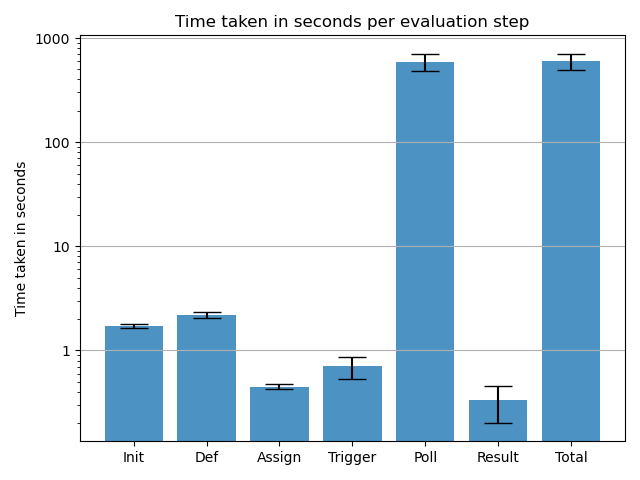
\includegraphics[width=15cm]{azure_evaluation_time.png}
\end{center}
\caption[Mean evaluation time of each phase with standard deviation plotted as bar chart]{Mean evaluation time of each phase with standard deviation plotted as bar chart}
%Source:
\end{figure}

The chart shows the mean run-time over 10 test runs for each phase as a separate bar. The black ranges indicated at the top of the bar charts display the standard deviation.
The Y-Axis indicates that all phases other than the polling - which includes the resource evaluation on Azure - can be ignored for this PoC. As mentioned before, the evaluation, as of now, trigger the whole suite of assigned policies instead of only one. Polling resides somewhere between 433 and 744 seconds. However, time not essential since executing the automated tests does not block SecurityRAT while the evaluation is going on.
In addition to that, explicitly triggering the evaluation of a single policy will decrease the run-time of the evaluation significantly. The function-based Config Rules in AWS \ref{awsConfigRules} have the advantage of being separately triggerable by nature, which results in a more suitable run-time.


\section{Response Check Microservice}
\label{refResponseCheckMS}
In contrast to the Azure microservice, run-time is not a significant concern of the Response Check microservice. As mentioned before, the company internal requirements are held very general, at least compared to, for example, the ASVS. This poses the difficulty of having a particular set of tests to be done in order to \enquote{Pass} a given requirement.

A possible solution for this has been described in \ref{customTestingScript}. By using a pseudo-database to map each requirement to a function that can hold any combination of tests according to the requirement, the problem of not having a clear definition of what has to be tested can be solved. In this case, an expert has to write the tests once. After that, they can be re-used for all other executions.

The implementation of this PoC only provides three examples based on the ASVS definition already used in \citep{secCat2020}, in a more abstracted and extendable manner. However, since the goal of this microservice is to test the feasibility of this approach and considering the vast diversity of requirement sets used in security compliance testing, providing an adaptable system is the main focus.

Further tests will show whether moving from a single, multi-requirement test to multiple, single-requirement tests pipeline will only increase the load of tasks, or deliver the expected advantages of further decoupling each requirement. This should avoid elongated executions or loss of state due to the blocking of short running evaluations or failing of evaluations. This refactor, of course, increases the work done by the gateway, which only should proxy the required evaluations to the microservices. For the scope of the PoC implemented in this thesis, this trade-off has been preferred.


\section{ZAP Microservice}
In order to test the ZAP microservice, run-time and result have been briefly analyzed to evaluate the feasibility of using an automated penetration testing tool as part of SecurityCAT.
The following tests have been done on the OWASP Juice Shop using the default settings for the ZAP Proxy. The default spider, Ajax spider, and active scanning have been used.
A crucial piece of information is that the \enquote{Runs} build on top of each other, meaning that the information found in the first run is used to conduct a more in-depth search in the second execution. This deepening of search space is prominent when looking at the \enquote{Runtime} row of the table. It indicates a possible exponential increase in run-time.

\newpage

\begin{table}[]
\begin{tabular}{|l|l|l|l|l|}
\hline
\textbf{Run}            & \textbf{1} & \textbf{2} & \textbf{3} & \textbf{4} \\ \hline
\textbf{Runtime (s)}    & 173.0392   & 314.6481   & 1054.3518  & 5688.1767  \\ \hline
\textbf{Alerts}         & 366        & 2799       & 11414      & 57176      \\ \hline
\textbf{Low}            & 137        & 1538       & 7587       & 41515      \\ \hline
\textbf{Medium}         & 129        & 936        & 3269       & 14877      \\ \hline
\textbf{High}           & 0          & 2          & 2          & 3          \\ \hline
\textbf{Grouped Alerts} & 10         & 13         & 13         & 13         \\ \hline
\textbf{Low}            & 5          & 6          & 6          & 6          \\ \hline
\textbf{Medium}         & 2          & 3          & 3          & 3          \\ \hline
\textbf{High}           & 0          & 1          & 1          & 1          \\ \hline
\end{tabular}
\caption{ZAP MS evaluation statistics}
\end{table}

With only one run, however, we were not able to find the \enquote{High} risk alert, which in this case, is a SQL Injection to log in as administrator.
This surfaces the problem that several executions might need to be executed in order to get any suitable result. Judging by the \enquote{explosion} of run-time over the four runs, this, however, is not feasible for the automation approach taken as part of this thesis.

Since the run-time escalation is a severe problem, for the scope of this thesis, no mapping has been implemented for the ZAP microservice yet. However, the mapping system introduced in \ref{refResponseCheckMS} provides a good baseline for further tests for the ZAP microservice.

As mentioned in \ref{drawbackAutomated}, automated penetration and vulnerability tests introduce a lot of false positives and are lacking the \enquote{expertise} of finding actual vulnerabilities.
Most results of ZAP only have a \enquote{medium} or \enquote{low} confidence level, which does not eliminate the need for manual checking and, therefore, reduce the benefit of such automated tests. 

The RAII (Resource allocation is initialization) principle, used in the creation process of new evaluations, works well for unauthorized API calls. A wrong API key instantly errors the evaluation and returns this status in the evaluation creation step. Therefore no evaluation session is started if the requester is not authorized.

In order to test the feasibility of using this automated penetration testing approach as part of the SecurityCAT setup, a demo application has to provide for tests in combination with the implemented internal requirements. Alternatively, additional tests with one of the famous test applications, like the OWASP Juice-Shop, can be conducted after an expert has analyzed it, and met requirements have been identified.


\section{Outlook}
The sections above already describe some of the drawbacks and potential points of failure of the implemented microservices. In addition to those, the full system has not been combined for testing. Each microservice was tested separately in combination with the gateway. Instead of SecurityRAT, the SwaggerAPI of the gateway was used to conduct the tests.
One of the next steps, therefore, is to combine SecurityCAT with SecurityRAT and run end-to-end tests for the whole pipeline.

One \enquote{drawback} of a microservice system are the many decoupled components. Starting and setting up the environment can be time-consuming and error-prone, repetitive work. By using containers and a docker-compose setup in the future, the whole system can be torn down and re-build automatically in no time.  

Additional thoughts have to be put into how to assign the requirement a more defined \enquote{YES} or \enquote{NO} according to the evaluation result. This concern is especially crucial for the ZAP and Response Check microservices. As described before, they carry a high chance of resulting low confidence results that could introduce more problems which, in the long run, would result in more work.